
\documentclass[]{article}
\usepackage{amsmath}
\usepackage{graphicx}
\graphicspath{ {images/} }
\begin{document}

\author{
  \textbf{ ABHISHEK GUPTA}
  \textbf{\textit{(2016CSJ0012)}}
}

\title{\textbf{Programming Practices \\Assignment 1\\Getting familiar with assembly language and ARMSim}}
\maketitle
\pagebreak
\section{Assumed Frequency}
Frequnecy= 1 $GHz$
\section{Instruction}
There are total 12007 number of instructions.
\section{Observed Time Elasped(According to computer)}
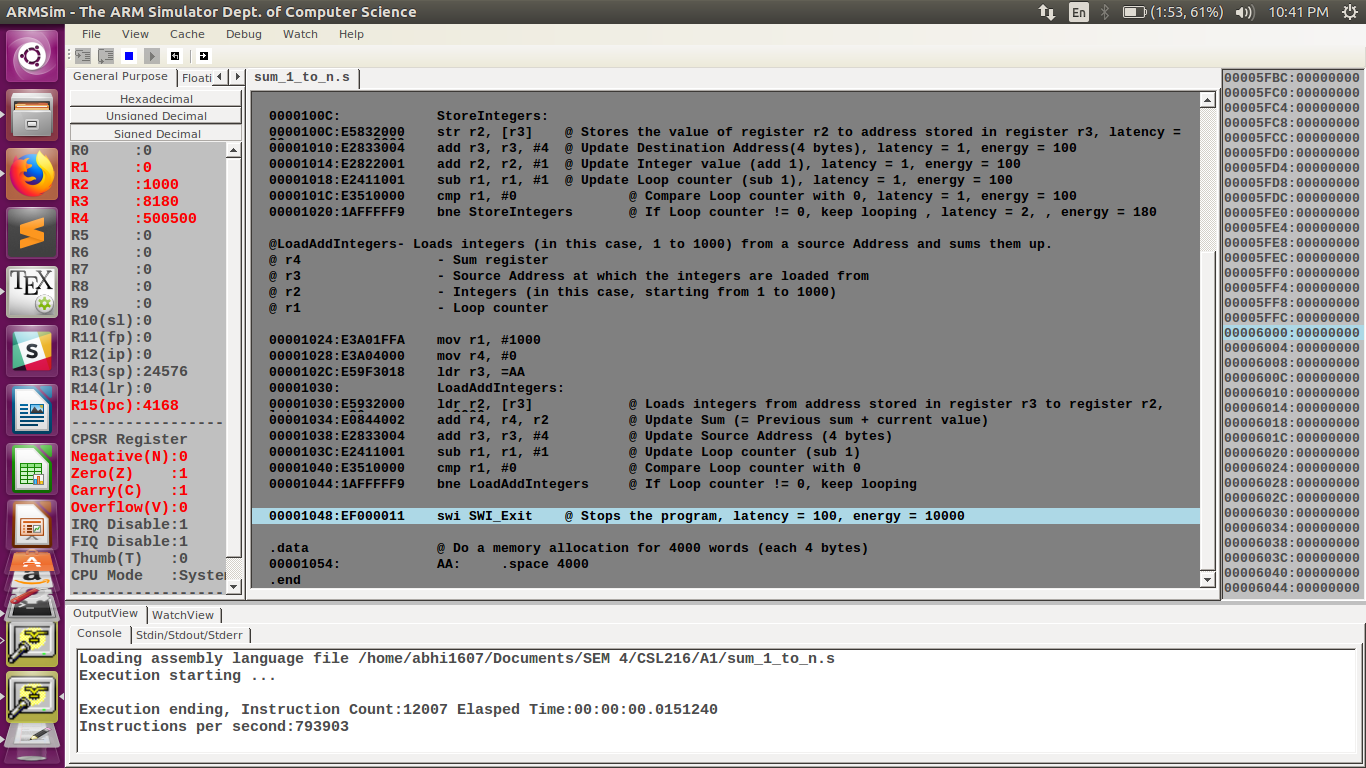
\includegraphics[scale=0.3]{screenshot}
Time Elasped is equal to $0.0151240$ $seconds$.
\section{Theoretical time elasped}
Theoretically time elasped = $\frac{Total Latency}{Frequency}=\frac{52106}{10^{9}}\frac{Cycles}{sec^{-1}}=5.21\times 10^{-5}$ $s$

\section{Total Energy}
The total energy is equal to $(100+100+110+(2000+100+100+100+100)*1000+1000*180+100+100+110+(2000+100+100+100+100)*1000+1000*180+10000) $\\$= 5170620 $   $pJ $ $  i.e.  $  $5.170620 \times 10^-6$  $J$.



\section{Total Latency}
The Total Latency is equal to $(1+1+1+1000*(20+1+1+1+1)+1000*2+ 1+1+1+1000*(20+1+1+1+1)+1000*2+100)=52106$ $cycles$.

\section{Theoretical Average Power Dissipation}
The Average Power Dissipation is equal to $\frac{{Total Energy}}{Theorectical Time Elasped}=\frac{5.170620}{52}\frac{\mu J}{\mu s} = 0.0994$ $ J/s $ \\$i.e.$ $ 0.0994$ $W $.
\section{Observed Average Power Dissipation}
The observed average power dissipation  $\frac{{Total Energy}}{Observed Time Elasped}=\frac{5.170620}{0.0159}\frac{\mu J}{s} $ $=325.19$ $\mu J/s$ $i.e $ $0.325\times 10^{-3}$ $J/s$
\section{Cycles per Instruction}
Cycles per Instruction=$\frac{Total Latency}{Total number of Instructions}$ = $\frac{52106s}{12007}\frac{Cycles}{Instruction}$ = $4.34$ $Cycles/Instruction$.
\\ \\ \\ \\ \\ \\ \\ \\ \\ \\ \\ \\ \\ \\ \\ \\ \\ \\ \\ \\
Copyright \copyright 6Feb --\the\year\ ABHISHEK GUPTA\par
NO Permission is granted to copy, distribute and\slash or modify 
this document under the terms \ldots. 

\end{document}